\documentclass{IEEEtran}
\usepackage[utf8]{inputenc}
\usepackage[english]{babel}
\usepackage{hyperref}
\usepackage{amsmath}
\usepackage{graphicx}
\usepackage{csquotes}
\usepackage{multirow}
\usepackage{graphics}
\graphicspath{{./images/}}
\usepackage[style=nature]{biblatex}
\addbibresource{references.bib}

\title{Assessing quality of music generated by the Music Transformer with an American Folk dataset \\
    \normalsize{\url{github.com/gregwinther/folk_transformer} and \url{https://gregwinther.github.io/folk_transformer/}}}

\author{\IEEEauthorblockN{Sebastian G. Winther-Larsen} \\
\IEEEauthorblockA{\textit{Center for Computing in Science Education,
    Department of Physics, University of Oslo} \\
}
\and
\IEEEauthorblockN{Tom F. Hansen} \\
\IEEEauthorblockA{\textit{Institute of Informatics, University of Oslo} \\
}
\and
\IEEEauthorblockN{Bjørn Iversen} \\
\IEEEauthorblockA{\textit{Institute of Informatics, University of Oslo} \\
}
}


\begin{document}
    \maketitle

    \begin{abstract}
        Since the publication of the music transformer in 2018, music generators based on
        the transformer architecture has been state of the art, making it possible to generate
        realistic music for minutes. Up to now the results have mainly been succesful for piano music, but
        have failed for more technically complex music such as jazz. Americana folk music can be seen as
        a stepping stone to more complex music. In this work we generate Americana folk music with 2 different approaches; transfer learning from the MAESTRO dataset and solely traning on the Americana dataset. We then evaluate these results in a qualitative and quantitative way. Results from the 
        quality assessment indicate that both models have been moderately succesful, and the model based on transfer learning is favoured. In a rating process people have rated the songs to in average 2.6,
         where 1 is not realistic and 5 is realistic, compared to "real" human-made music. In a technical 
         evaluation the evaluated songs showed a....
        \end{abstract}
        
        \begin{IEEEkeywords}
        music generation, transformer model, evaluation, transfer learning, Americana
        \end{IEEEkeywords}

    \section{Motivation and introduction}

        The attention-based transformer model \cite{vaswani2017attention},
        is today recognised as the best performing sequential machine learning model,
        surpassing RNN-based models in most cases, mainly argued by its better abilities
        to remember long term coherence, shorter training time and applicability in transfer
        learning. While originally used primarly for
        natural language processing (NLP), which today has mature implementations,
        the architecture can also be applied for other sequential learning tasks,
        such as music generation~\cite{huang2018music}.
        The music transformer developed in the Magenta project is trained on the Maestro
        dataset~\cite{maestrodataset}.
        By setting a primer – a start music sequence, the model generates new music with good
        results along the same lines as the training set. With other primers than the regular and
        systematic classical music in \textbf{MAESTRO}, the quality of the output is varying.

        Motivated by generating more irregular music, \emph{the main goal} of the work is
        to describe a framework for the quality assessment of different approaches to the generation 
        of music with the transformer model. We compare two different Transformer implementations and use our proposed evaluation framework to assess 
        the quality of each approach. It is not known to the authors scientific papers
        describing such a comparison of music transformers.
        At the core of such an evaluation framework is, for each approach; a) in order to make a fair comparison,
        a detailed description of model topology, its tuning parameters, and the size
        and structure of the dataset used for training, and b) an evaluation format
        that combines a form of quantitative and qualitative evaluation technique.
       
        To this end, we wish to employ the transformer music to a subgenre of music   
        to which such a model has not been extensively applied.
        Initial findings from applying the transformer to jazz music has shown 
        some limitations~\cite{wu2020jazz}, applying LSTM networks to Blues has 
        been moderately succesful~\cite{eck2002bluesLSTM} and applying the transformer 
        model to pop music seems to work well~\cite{huang2020pop}.
        From a music theory standpoint this is very sensible - classical music often has 
        formal rules, the epitome of which is the fugue~\cite{giraud2015computational};
        and pop music follows some very clear norms~\cite{hennion1983production}. While 
        even Free Jazz has \emph{some} rules, it readily falls into the category of the 
        type of rhytmic music with the least amount of structure, per the definition
        that it is ``characterized by the absence of set chord patterns or
        time patterns''\cite{FreeJazz}. 

        American roots music, encompassing spirituals, cajun music, cowboy music, work songs,
        but also early blues such as Dixieland; from now on referred to as ``Americana'', presents 
        itself as hitherto unexplored territory. It also provides a nice stepping stone
        towards more ``unstructured'' music as it often allows for improvisation, but 
        otherwise retains a relatively rigid structure~\cite{libcong}.
        We have therefor collected a dataset of MIDI files of Americana music, which we
        will use in our quality assessment framework. \emph{A second goal}, but less important in light of the main motivation is therefore to realisticly generate Americana music with the transformer architecture. \emph{A natural aim} in the process-steps is to investigate the superiority of music generators based on a significantly higher number of songs, even though this could be music from other genres, by utilizing transfer learning from the \textbf{MAESTRO} dataset in the music transformer \cite{huang2018music}. The 3 goals are tightly interconnected, typicly superseeding each other in process-steps.

    \section{Related work}
       The transformer model is considered state of the art in music generation,
       surpassing RNN-based models in the last few years. Both are sequential models,
       but the attention principle at the core of the transformer facilitates
       remembering coherence over longer sections of sequences and highlights
       especially important sections. From generating music of 10's of seconds with RNN, it is now possible to generate a minute of coherent realistic music ~\cite{huang2018music}. Still there is a lot of unresolved challenges, like generating long sections (over some minutes), in highly irregular compositions
       and multi channel (many instruments) signals. To combat these challenges the
       improvement of the transformer model has high focus in the research community.
       Some of the most recent attempts are the Transformer-XL~\cite{dai2019transformerxl} 
       model and the Reformer~\cite{kitaev2020reformer} as particularly promising
       candidates.
       A Reformer model claim to be trained on a standard computer with a single GPU.
       In this analysis we will utilize the original transformer architecture, as this
       is the model-architecture in the music transformer from Google.

       \subsection{Music transformers}
       In the few existing papers considering music generation with the Transformer
       we want to emphasize some important related works besides the beforementioned
       music transformer, built on the classical piano music dataset MAESTRO.
       These works are somewhat diversified in different music genres, describing the span of existing music genres generated by the transformer, "setting the stage" for the Americana music in this work. In the pop
       music transformer \cite{huang2020pop} pop piano music is generated by the
       transformer, a setting quite similar to the classical piano music in \cite{huang2018music}. 
       %The paper shows that Transformers can do even better for music
       %modeling, when the way a musical score is converted into the data fed to a
       %Transformer model, is improved. This is performed by imposing a metrical structure
       %in the input data, so that Transformers can be more easily aware of the
       %beat-bar-phrase hierarchical structure in music. The new data representation
       %maintains the flexibility of local tempo changes, and provides hurdles to control
       %the rhythmic and harmonic structure of music. With this approach, this work
       %claims to generate pop piano music with better rhytmic structure than the music
       %transformer \cite{huang2018music}.

       Another paper describes the Jazz transformer~\cite{wu2020jazz} which is in the
       other end of the spectrum related to complexity. Here the the Transformer-XL
       architecture is utilized to model lead sheets of jazz music. Moreover, the model
       endeavors to incorporate structural events present in the Weimar Jazz Database
       (WJazzD) for inducing structures in the generated music. Even though the training
       loss values are low, the esults are not impressive. Listening tests shows a clear
       gap between the ratings of the generated and real compositions. The work analyses
       the missing parts and presents a prediction system which in an analytical manner
       shed light on why machine-generated music to date still falls short of the artwork
       of humanity. This includes analyzing the statistics of
       the pitch class, grooving, and chord progression, assessing the structureness of
       the music with the help of the fitness scape plot, and evaluating the model’s
       understanding of Jazz music. The evalutation scheme and the failure to generate such complex music is relevant in the generation of Americana.

       In a system called LakhNES~\citeauthor{donahue2019lakhnes},
       generate multi-instrumental music with the transformer~\cite{donahue2019lakhnes}.
       Their success of music generation with the piano score generation is partially
       explained by the large volumes of symbolic data readily available for that domain.
       They leverage the recently-introduced NES-MDB dataset of four-instrument scores
       from an early video game sound synthesis
       chip\footnote{The Nintendo Entertainment System (NES)}.
       They found this data to be well-suited to training with the
       Transformer architecture. The model was further improved with a pre-training
       technique to leverage the information in a large collection of heterogeneous music,
       namely the Lakh MIDI dataset. By performing transfer learning on the NES-MDB dataset,
       both the qualitative and quantitative performance from the target dataset was
       significantly improved. The rare use transfer learning in music generation with the transformer is a relevant foundation for use of transfer learning in this work.
       
        \citeauthor{gan2020foley} use
        the transformer architecture to generate music, but with another approach.
        In a system called Foley Music they synthesize music from a silent video about
        people playing instruments~\cite{gan2020foley}.
        A relationship between body keypoints and classical MIDI recordings is established.
        Music generation is then formulated as a motion-to-MIDI translation problem,
        represented with a graph transformer framework that predict MIDI from motion.
        By testing the generator on different music performances the results is proven to outperform several existing systems in music generation.

        However, there is little work on generating intentionally the same music generator
        with different approaches. Another new approach is to use transfer learning from
        an existing high performance music model.

        \subsection{Evaluation of ML-generated music}
        In the evaluation of models of music generation based on machine learning we
        would like to point out the works by \citeauthor{1030094}~\cite{1030094},
        \citeauthor{yang2020evaluation}~\cite{yang2020evaluation}
        and \citeauthor{wu2020jazz}~\cite{wu2020jazz}.
        These works describe either a qualitative evaluation or a qualitative evaluation.
        In our attempt we combine these 2 approaches and establish a common framework.

    \section{Methods}

        Acting as a base and for exemplification of the benchmark architecture,
        Americana music is generated in 2 different model concepts:
        \begin{enumerate}
            \item Utilize transfer learning with MAESTRO music transformer as a base,
                    and train with the full dataset of Americana midi-files (hereafter called Transfer Americana).
            \item Train a new transformer model only using the full Americana dataset (hereafter called Americana)
        \end{enumerate} 
        
        A hypothesis is that concept number 1 will result in the best performing model,
        but an important issue is what makes up the best model and how to evaluate such a
        subjective "sequence-result" as music in a fair and trustworthy manner? 
        Some will say this is an impossible task ~\cite{1030094}. Will a transfer learning model be significantly better than only training on a single dataset, such as has been shown in other ML-applications, like image classification \cite{7404017}, even though the MAESTRO dataset is totally different from the Americana dataset.

        An attempt to sort this out is by evaluating in a quantitative and qualitative way.
        The quantitative, hence objective, way can shortly be described as a technical
        comparison of the predicted signal and the real signal. Principles by \cite{yang2020evaluation} and ~\cite{wu2020jazz} will be utilized.
        
        The qualitative part constitutes a music expert judgement,
        based on listening to the generated music files from the objective evaluation.
        In a second, and survey based part, a number of random people is asked
        to rate the different music files.
        
        \subsection{Modelling process}
        MIDI-files was first preprocessed to fit into the format used by the transformer model.
        This was carried out by utilizing an implementation of a transformer adapted for music, 
        incorporated in a package from Musicautobot \cite{musicautobot}. Scripts for transfer learning and
        single learning were built around this package. Both models had the same model topology, used the same tuning parameters, and were trained on a supercomputer at University of Oslo
        with the following specification for xxx hours:
        %TODO: sebastian fyller du inn. Benedicte ville gjerne ha beskrevet workflow.

        \subsection{Qantitative evaluation}
        
        For quantitative evaluation, we will be using the objective
        evaluation toolbox mgeval~\cite{yang2020evaluation}.
        The toolbox let us extract absolute metrics from MIDI files
        which let us inspect the properties of both the dataset used
        for training and the generated dataset. The features extracted
        for absolute measures are divided into pitch-based features Pitch count (PC),
        Pitch class histogram (PCH), Pitch class transition matrix (PCTM),
        pitch range (PR) and Average pitch interval (PI) and rhythm-based features,
        Note count (NC), Average inter-onset-interval (IOI), Note length
        histogram (NLH) and Note length transition matrix (NLTM).
        These metrics can then be used to acquire the relative metrics between
        datasets with the use of exhaustive cross-validation to acquire the
        distance between each sample of the same set (intra-dataset) and another
        set (inter-dataset). 
        
        \subsection{Evidence-Based Design for Assessment and Evaluation}
        As a rigorous and well-proven approach do construct a framework for 
        assessing music composed by artificial intelligence models, we propose 
        adapting the methodology of Evidence-Centered
        Design~\cite{mislevy2003focus,mislevy2017evidence}
        By working with Evidence-Centered Design (ECD), we engage in a modern
        approach to assessment design,
        for assessing complex knowledge and practices.
        ECD is originally applied to the contruction of psychometric learning
        assessment tools. Through to completion, it would take several years to 
        construct such a tool, something that is well outside the scope of this 
        study. However, we prospose to begin with the first step within ECD - 
        \textbf{Domain Analysis}. This involves exploratory interviews of experts
        in the field in order to contruct a thematically organized and prioritized
        list of knowledge and practices to assess. Specific to our study,
        we find it necessary to talk to professional musicians and composers 
        in order to uncover what actually makes a good composition.
        
        In a second part of the qualitative evaluation a survey was carried out, involving random people with random background. Pople were presented to 5 generated songs with length 
        40 seconds - 1 minute, facilitated in a Google survey form. The songs were generated by sending a primer of the first 3 bars (5 seconds) of 5 different original songs from the Americana dataset to the trained model. Each song were presented in 2 versions, one generated  by Transfer-Americana and one by Americana. They had to choose the one they liked best in each pair of songs. In addition they 
        had to rate the best version related to how realistic it was compared with human 
        generated music. The range was 1-worst to 5-best.

    \section{Datasets}

        A brief summary of each of the datasets we have used in this study 
        can be found in \autoref{tab:data}.

        \textbf{MAESTRO}~\cite{maestrodataset}
        (MIDI and Audio Edited for Synchronous TRacks and Organization)
        is a dataset with over 200 hours of virtuosic piano perfomances captured with 
        a fine alignment of approximately 3ms between note lables and audio waveforms.

        The data is a produce from performances in the International Piano-e-competition.
        During each installment of the competiton, virtuoso pianists perform on Yamaha
        Disklaviers which, in addition to being concert-quality acoustic grand pianos,
        utilize integrated high-precision MIDI capture and playback.
            
        Since the \textbf{MAESTRO} dataset contains MIDI recordings from competions, 
        the pieces are from a select set for each year. This means that many of the 
        pieces are the same, but may includes much variation within each
        performer's interpretation of the piece. 

        The \textbf{Americana} dataset is constructed from musical scores by 
        Benjamin Robert Tubb\footnote{These were scraped from a webpage that has 
        since been taken down. Consequently, we are unable to provide a proper 
        reference}. These scores are in the public domain and composed between
        the ealry 1800s and 1922. The genres range from blues, ragtime, naval songs,
        hyms, minstres songs and spirituals. 
    
        \begin{table}
        \begin{center}
            \caption{Data set description \label{tab:data}}
            \begin{tabular}{l c c c} \hline
                & MAESTRO v2 & Americana \\ \hline\hline
            No. of songs & 1282 & 5711 \\ \hline
            Total time [hours] & 201 & 329 \\ \hline
            Mean length [min] & 9.4 & 3.45  \\ \hline
        \end{tabular}
        \end{center}
        \end{table}



    \section{Results}

    \subsection{Quantitative evaluation}
        \begin{table}
            \begin{center}
            \caption{
                Results from relative measurements of Intra-set distances.
                \label{tab:q_results}
            }
            \begin{tabular}{l|rr|rr|rr}
            \multirow{3}{*}{} &
            \multicolumn{2}{c|}{Training} &
            \multicolumn{2}{c|}{Americana} &
            \multicolumn{2}{c}{Transfer} \\ \cline{2-7} 
            &
            \multicolumn{2}{c|}{Intra-set} &
            \multicolumn{2}{c|}{Intra-set} &
            \multicolumn{2}{c}{Intra-set} \\ \cline{2-7} 
            &
            \multicolumn{1}{c|}{mean} &
            \multicolumn{1}{c|}{STD} &
            \multicolumn{1}{c|}{mean} &
            \multicolumn{1}{c|}{STD} &
            \multicolumn{1}{c|}{mean} &
            \multicolumn{1}{c}{STD} \\ \hline
            PC   & 11.777  & 1.700  & 3.577  & 0.636 & 6.466  & 0.706 \\
            NC   & 442.377 & 73.911 & 11.377 & 1.542 & 21.955 & 4.678 \\
            PCH  & 0.384   & 0.013  & 0.164  & 0.007 & 0.365  & 0.026 \\
            PCTM & 821.396 & 56.336 & 10.475 & 0.292 & 25.991 & 3.303 \\
            PR   & 19.088  & 1.638  & 5.266  & 0.611 & 10.400 & 2.038 \\
            PI   & 3.836   & 0.510  & 0.848  & 0.128 & 2.032  & 0.479 \\
            IOI  & 0.046   & 0.006  & 0.105  & 0.007 & 0.235  & 0.022 \\
            NLH  & 0.471   & 0.027  & 0.263  & 0.022 & 0.466  & 0.043 \\
            NLTM & 316.896 & 23.442 & 23.241 & 1.359 & 46.778 & 4.027
            \end{tabular}
            \end{center}
            \end{table}

            \begin{figure}
                \centering
                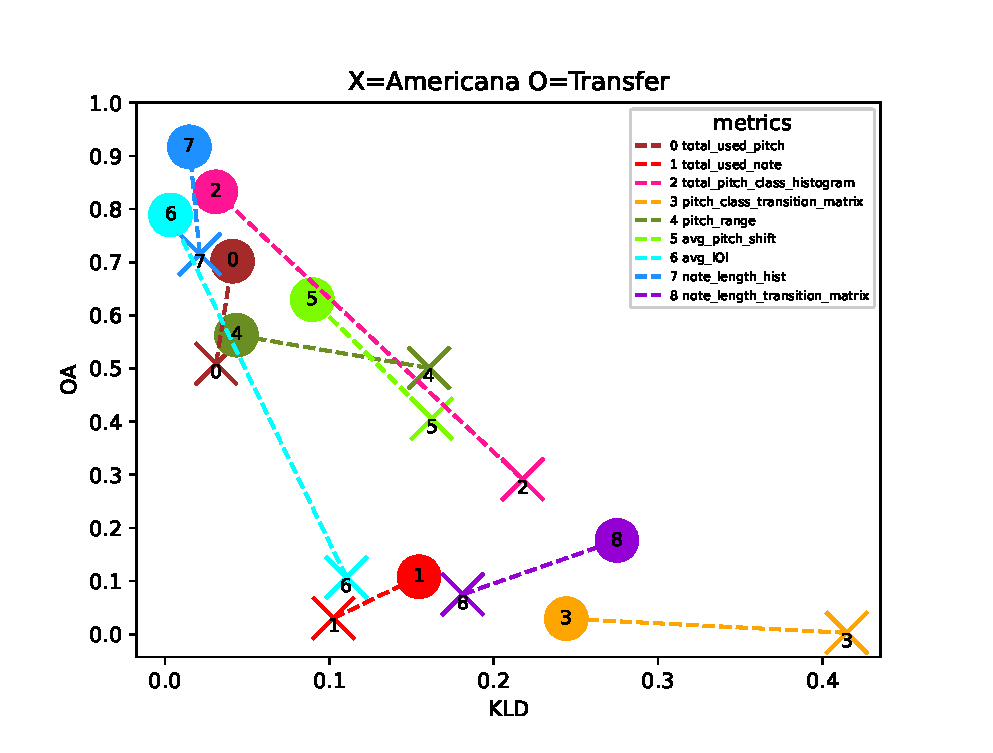
\includegraphics[width=8.5cm, height=5cm]{gen_intra_gen_training_inter}
                \caption{Visualisation of the KLD and OA of the Intra-set generated from Training set and the American/Transfer sets.}
                \label{fig:gen_intra_gen_training_inter}
            \end{figure} 
            
            \begin{figure}
                \centering
                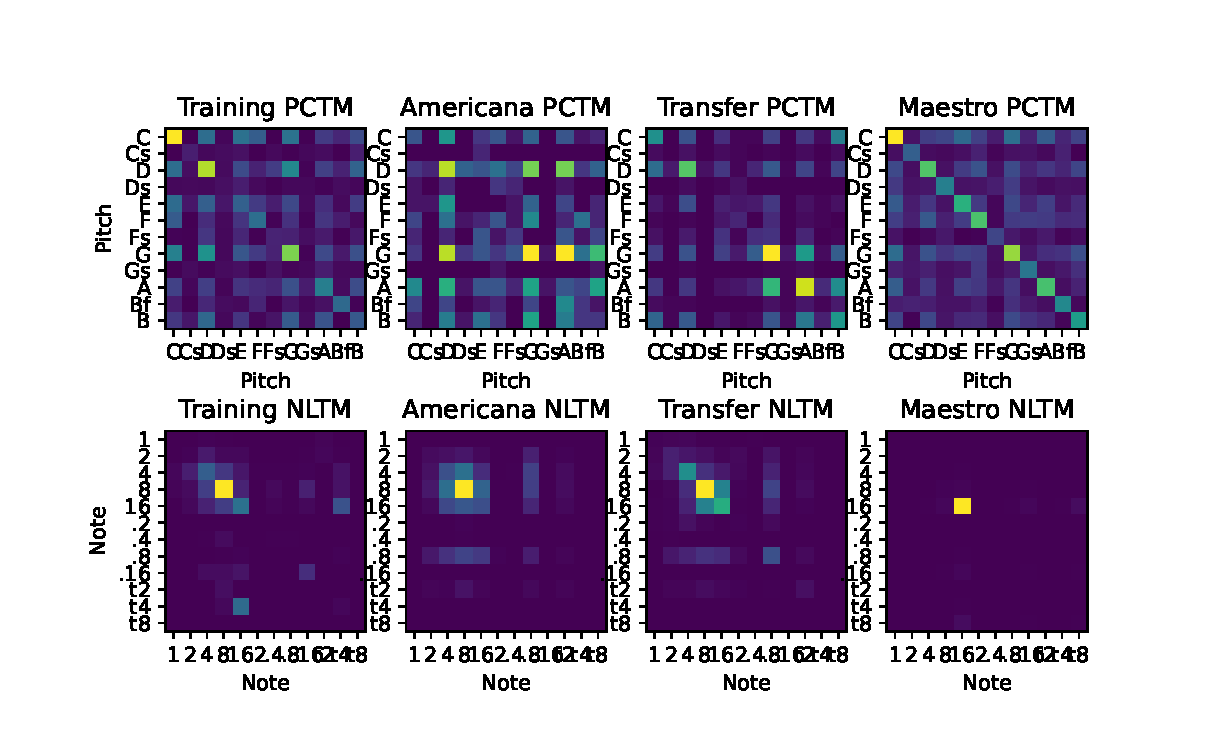
\includegraphics[width=8.5cm, height=5cm]{PCTMNLTM.eps}
                \caption{Absolute measurements of average pitch class transition matrix (PCTM) and note length transition matrix (NLTM) from the Americana training set, Americana generated, transfer generated and maestro training set (sect IV.A.)}
                \label{fig:absoluteNLTMPCTM}
            \end{figure} 
         
            For this evaluation we have picked 10 melodies from both the Americana dataset and the Maestro dataset, as well as using 10 different primers to generated 10 melodies with the Americana trained and the transfer trained sets. 

            The results for the absolute measures of note length transition matrix \ref{fig:absoluteNLTMPCTM} shows us that the Americana/training dataset have a greater variety in note length than the maestro set. We can see that the melodies generated with the Americana dataset have similar variety, and that the melodies generated Transfer set influenced by the maestro set preservers most of variety. The result for pitch class transition matrices on the other hand shows a decrease in variety in the transfer generated song.

            The results for the relative measurements shown in table \ref{tab:q_results} and figure \ref{fig:gen_intra_gen_training_inter}. From the comparisons we can see that both the Americana and Transfer sets have notably smaller mean values in the Intra-set across the board, apart from average inter-onset-interval (IOI). This does imply that there is less variation in the generated samples than the training set, while the time between each note also increases as seen in the IOI. We can also see that the transfer set does have twice as high mean than the Americana set which does indicate notable improvements in the generated melodies, however the standard deviation increases as well which implies that the mean in the transfer set is less reliable.
            
            Lastly, we will look at the Kullback–Leibler divergences (KLD) and Overlapping area (OA) for the Inter-sets generated for training-Americana and training-transfer as seen in figure \ref{fig:gen_intra_gen_training_inter}. We can see that the OA for the transfer set is greater for all the metrics which again indicates improvements in transfer over the Americana set. However, there is also an increase in the KLD for pitch count, note count and note length, which indicates that these metrics are less reliable.
        

    \subsection{Qualitative evaluation}
    
        \begin{figure}
            \centering
            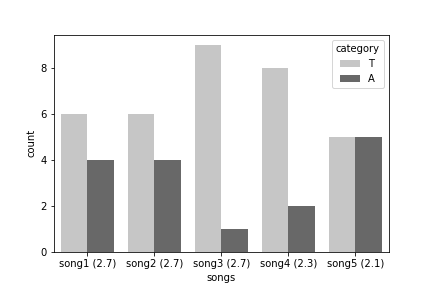
\includegraphics[width=8.5cm, height=5cm]{songs_category.png}
            \caption{Bars show a count of the number of votes, respectively for Transfer-Americana
             and Americana, for each of the 5 songs. The numbers in parenthesis below the Bars
             is the average rating for each of the songs, when compared to a realistic human made
             song (1 is worst, 5 is best)}
             \label{fig:songs}
        \end{figure} 

        \begin{figure}
            \centering
            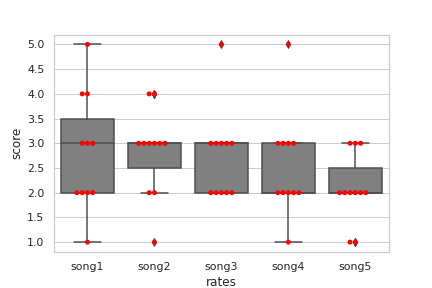
\includegraphics[width=8.5cm, height=5cm]{scores.png}
            \caption{Boxplot of ratings for each of the 5 songs when compared to a realistic human made song (1 is worst, 5 is best). Median in horisontal black line, box defines by 25-75 percentile. The red dots are all registered scores.}
             \label{fig:scores}
        \end{figure} 

        Figure \ref{fig:songs} visualize a count of the number of votes, respectively for Transfer-Americana
        and Americana, for each of the 5 songs. The numbers in parenthesis below the Bars is the average rating for each of the songs when compared to a real human-made song (1 is worst, 5 is best). Inspecting the figure we see a general trend where Transfer-Americana is favoured in 4 of 5 songs. Song 5 has a closer score and is also the song with the lowest average rating of 2.1. 69 \% of all choices favour Transfer-Americana. A t-statistic was calculated for this result, describing a significant favouring of 
        Transfer-Americana, with a p-value of 0.07. These results verified the hypothesis that a music transformer model will perform better when it is based on the pre-trained model, increasing the total number of music-samples, even though the base model was trained on the classical \textbf{MAESTRO} dataset. It must be pointed out the uncertainty related to the relatively low number of samples in the survey. 
        In figure \ref{fig:scores} a boxplot is visualizing the single scorings in a more detailed manner. Red points marks all the single scorings. The median for song 1-4 has a score of 3 and also single scorings of 4 and 5, indicating that some people consider the songs as comparable to human made music.
        
        In this survey some people have made comments about the overall performance, focusing more on the subjective experience. We bring some of the more noteworthy comments:
        \begin{enumerate}
            \item \emph{The songs appear to all get worse the longer they go on, as in the notes get more sparse and less cohesive. They both also has a thing of really going all the way through a scale, playing every note, to get somewhere...These two things make it very clear it is not a trained human playing}
            \item \emph{There appeared to be some strange audio artefacts (reverb/echo-like) on a few of the tracks, particularly transfer americana 2.
            Also, it might have been better if the songs from the different generators were shuffled for each question, so we didn't naturally consider the differences between the two}
            \item \emph{Which song is made by which algorithm should be secret, as it will colour our opinions. You should also clearly state what the scale from 1 to 5 is meant to be ranging across. Is it for instance meant to be from "clearly a robot has made this" to "could be made by an expert composer"?}
        \end{enumerate}

        Evaluation carried out in interview with musicians resulted in.... %TODO: Sebastian

    \section{Discussion}
    When we compare the results from the quantitative and qualitative evaluation we see the same trend ..

    Important goals of the work was 1) to verify that a model trained by transfer learning and therefore based on more samples will perform better, even though the base model constitute of songs of a different music genre, and 2) show that it is possible to generate more complex music than generated in earlier related work. Results from qualitative and quantitative evaluation clearly shows that Transfer-Americana perform better than Americana, fullfilling goal 1). Scorings from comparison with human-made music to some degree supports goal 2), with an average rating of 2.6 of 5, but there is still a way to go. Especially for the songs from the Americana model, we see that the melodic part degrades faster than for Transfer-Americana, a pattern wich probably has affected the comparisons and the scoring.

    An interesting pattern is the variation in count of superiority between songs in figure \ref{fig:songs}. In song 1-4 the count shows a clear overweight on Transfer-Americana, especially evident for song 3 and 4. For song 5 the count is close to similar. When we compare this to the technical evaluation we see the same pattern TODO: It could be that the composition and complexity in certain primers is more dependent on a bigger database of trained songs, than other primers. This is something to further analysis i future work. Scorings in figure \ref{fig:scores} returns many 3's and some 4's and 5's, but also 1's, indicating that some people think this is truly realistic music, while others condider human-made and generated music as two different worlds.

    A third goal was to suggest a scheme for evaluating of music generated music. The combination of a quantitative system and two approaches of qualitative evaluation gives a broader view of the results, also touching upon the more subjective parts of an evaluation. The consistency of resuls over these evaluation forms gives a higher confidence in a total evaluation-result.

    
    \section{Conclusions and further development}
    Combining the evaluation metrics in a more schematic way, possibly classifying generated music in classes based on input values as; music genre, personal listening-profile (musical background etc.). 

    \vfill
    \pagebreak
    \printbibliography
\end{document}
